
\section{Layered Topological Organization}
\label{sec:layered_dag_traversal}

Recall that a \acrshort{pdag} \(\mathcal{G} = (\mathcal{V}, \mathcal{E})\) contains no cycles, so there is at least one valid \emph{topological ordering} of its nodes.  A topological ordering assigns each node a numerical \emph{layer index} such that all edges point from a lower-numbered layer to a higher-numbered layer. If a node \(v\) consumes the outputs of nodes \(\{u_1,\dots,u_k\}\), then we require
\[
\text{layer}(u_i) \;<\; \text{layer}(v)
\quad
\text{for each }i\in\{1,\dots,k\}.
\]
In other words, node \(v\) can appear only after all of its inputs in a linear or layered listing.

The essential steps to build and traverse these layers are:

\begin{enumerate}
    \item \emph{Compute Depths via Recursive Analysis:}  
      Each node's depth is found by inspecting its children (or inputs).  If a node is a leaf (e.g., a \texttt{Variable} or \texttt{Constant} that does not depend on any other node), its depth is 0.  Otherwise, its depth is one larger than the maximum depth among its children.  

    \item \emph{Group Nodes by Layer:}  
      Once each node's depth is computed, nodes of equal depth form a single \emph{layer}. Thus, all nodes with depth \(0\) are in the first layer, those with depth \(1\) in the second layer, and so on.  

    \item \emph{Sort Nodes within Each Layer:}  
      Within each layer, enforce an additional consistent ordering: (i)~variables appear before gates, (ii)~gates of different types can be grouped to facilitate specialized processing.  This step is not strictly required for correctness, but it can streamline subsequent stages such as kernel generation or partial evaluations.

    \item \emph{Traverse Layer by Layer:}  
      A final pass iterates over each layer in ascending order.  Because all inputs of any node in layer \(d\) lie in layers \(< d\), the evaluation (or "kernel build") for layer \(d\) can proceed after the entire set of layers \(0,\dots,d-1\) is processed.
\end{enumerate}

This structure ensures a sound evaluation of the \acrshort{pdag}: no gate or variable is computed until after all of its inputs are finalized.

\begin{figure}
    \centering
    \begin{subfigure}{1\textwidth}
        \centering
        \includesvg[height=0.3\textheight]{figs/pdag/dag_pass_1.svg}
    \caption{Working example from Fig.~\ref{fig:pdag_pass_1}.}
        \label{fig:recall_pdag_pass_1}
    \end{subfigure}
    \vfill
    \begin{subfigure}{1\textwidth}
        \centering
        \includesvg[width=0.6\linewidth]{figs/pdag/dag_pass_2.svg}
        \label{fig:pdag_pass_2}
    \end{subfigure}
    \caption{Layered topological ordering on the Propositional \acrfull{dag}, with coalesced/fused kernels, partitioned by operation type.}
\end{figure}

\subsection{Depth Computation and Node Collection}

\begin{enumerate}
    \item \textbf{Clear Previous State.}  
      Any existing "visit" markers or stored depths in the \acrshort{pdag}-based data structures are reset to default values (e.g., zero or -1).
      
    \item \textbf{Depth Assignment by Recursion.}  
      A \texttt{compute\_depth} subroutine inspects each node:
      \begin{enumerate}
        \item If the node is a \texttt{Variable} or \texttt{Constant}, it is a leaf in the \acrshort{pdag}, so depth \(=0\).  
        \item If the node is a \texttt{Gate} with multiple inputs, the procedure first recursively computes the depths of its inputs. It then sets its own depth as 
        \[
          \text{depth}(\texttt{gate})
          \;=\;
          1 \;+\;\max\limits_{\ell \in \text{inputs of gate}} \Bigl[\text{depth}(\ell)\Bigr].
        \]
      \end{enumerate}
    \item \textbf{Order Assignment.}  
      Each node stores the newly computed depth in an internal field. This numeric value anchors the node to a layer. A consistent pass over the entire graph ensures correctness for all nodes.
\end{enumerate}

After depths are assigned, gather all nodes, walking the \acrshort{pdag} from its root, recording each discovered node and adding it to a global list.

\subsection{Layer Grouping and Local Sorting}

Begin by creating:
\begin{itemize}
\item A global list of all nodes, each with a valid depth,  
\item A mapping from node indices to node pointers,  
\end{itemize}
Then, sort the global list by ascending depth.  Let \(\text{order}(n)\) be the depth of node \(n\).  Then
\[
\text{order}(n_1)\;\le\;\text{order}(n_2)\;\le\;\dots\,\le\;\text{order}(n_{|\mathcal{V}|}).
\]
Finally, partition this list into contiguous \emph{layers}: if the deepest node has a depth \(\delta_{\max}\), then create sub-lists:
\[
\{\text{nodes s.t. depth}=0\},
\quad
\{\text{nodes s.t. depth}=1\},
\quad
\dots,
\quad
\{\text{nodes s.t. depth}=\delta_{\max}\}.
\]
Within each layer, sort nodes to ensure that \texttt{Variable} nodes precede \texttt{Gate} nodes, and \texttt{Gate} nodes may be further sorted by \texttt{Connective} type (e.g., \texttt{AND}, \texttt{OR}, \texttt{VOT}, etc.).

\subsection{Layer-by-Layer Kernel Construction}

Apply the layer decomposition to drive \emph{kernel building} and \emph{evaluation}:

\begin{enumerate}
    \item \textbf{Iterate over each layer in ascending depth}.  Because every node's dependencies lie in a strictly lower layer, one is guaranteed that those dependencies have already been assigned memory buffers, partial results, or other necessary resources.
    \item \textbf{Partition the layer nodes into subsets by node type}.  Concretely, \texttt{Variable} nodes are batched together for \emph{basic-event sampling} kernels, while \texttt{Gate} nodes are transferred into \emph{gate-evaluation} kernels.  
    \item \textbf{Generate device kernels}.  For \texttt{Variable} nodes, create Monte Carlo sampling kernels. For \texttt{Gate} nodes, it constructs logical or bitwise operations that merge or transform the sampled states of the inputs.  
\end{enumerate}

Once kernels for a given layer finish, move on to the next layer. Because of the topological guarantee, no node in layer \(d\) references memory or intermediate states from layer \(d\!+\!1\) or later, preventing cyclical references and ensuring correctness.


\section{Adopting the SYCL Execution Model}

Before getting into our opinionated launch parameters, it is instructive to recall the abstract execution hierarchy defined by the SYCL standard. This detour provides the conceptual foundation upon which the remainder of this dissertation builds.

\begin{figure}[hb]
    \centering
    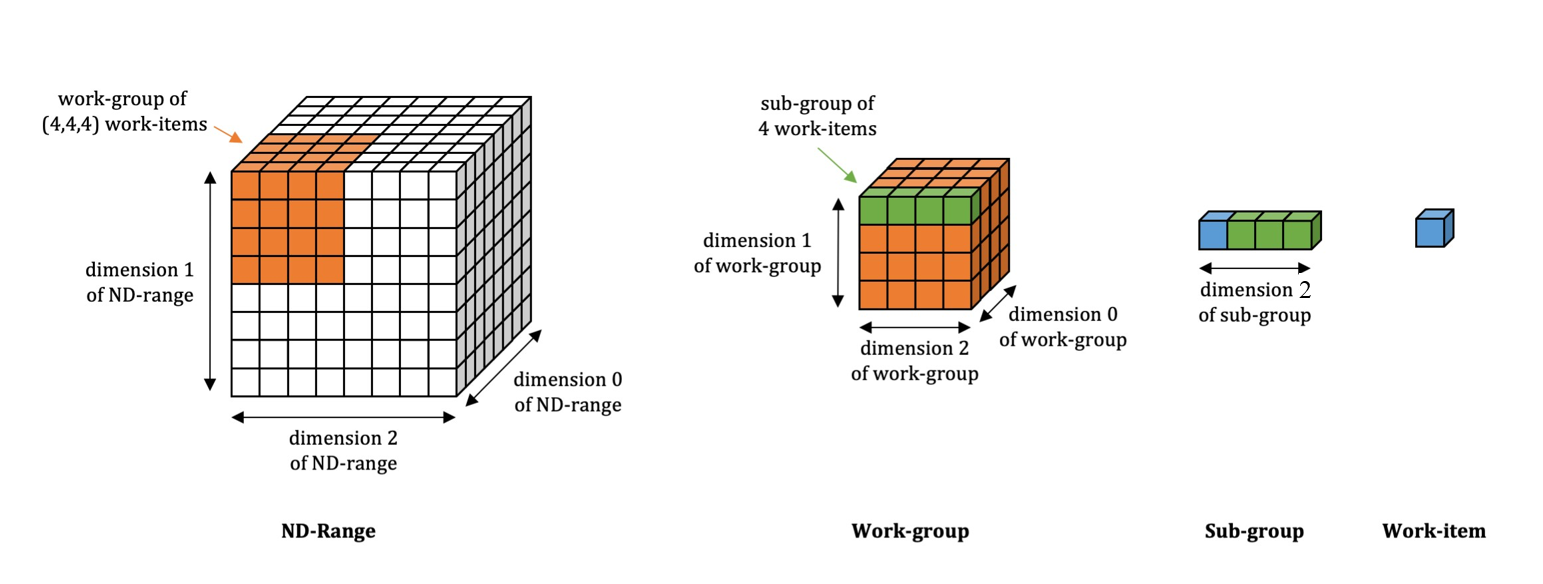
\includegraphics[width=1\textwidth]{figs/sycl/sycl_execution_model.png}
    \caption{At a glance: The SYCL execution model describes relationships between ND-Ranges, work-groups, sub-groups, and work-items.}
    \label{fig:sycl_exec_model}
\end{figure}

% -----------------------------------------------------------------------------
%  Conceptual overview and formal relationships
% -----------------------------------------------------------------------------
\subsection{Conceptual Overview}  Modern accelerator programming models must present the developer with a 
\emph{logical} view of parallel work that is independent of any specific piece of hardware.  SYCL achieves this
by defining a small hierarchy of index spaces.  Each level in the hierarchy provides progressively stronger 
coherence and synchronization guarantees, yet none of them prescribes 
\textit{where} that work will eventually run.  The mapping from logical indices to physical execution resources is
entirely deferred to the run--time or device compiler and is therefore opaque to the application.  In what follows we formalize the four key abstractions exposed by the SYCL execution model and derive a set of identities that will be reused throughout the remainder of this dissertation.

\subsection{Hierarchical Index Spaces}  Let
\[
   \mathbf{G} = (G_x,G_y,G_z) \in \mathbb{N}^3, \qquad
   G_d > 0\quad(d\in\{x,y,z\}) ,
\]
be the \emph{global range}.  It enumerates the total number of logical tasks, or \emph{work--items}, that shall be executed in one kernel invocation.  The associated set of global indices is
\[
    \mathcal{I} \;=\; \{0,\dots,G_x-1\} \times \{0,\dots,G_y-1\} \times \{0,\dots,G_z-1\},
\]
with
\( |\mathcal{I}| = G_x G_y G_z. \)

A second triple
\[
    \mathbf{L} = (L_x,L_y,L_z), \qquad 0 < L_d \le G_d ,
\]
referred to as the \emph{local range}, partitions the ND--Range into disjoint \emph{work--groups}.  Defining
\[
    W_d \;=\; \frac{G_d}{L_d},\qquad d\in\{x,y,z\},
\]
(which implies $G_d \equiv 0\; (\mathrm{mod}\,L_d)$), the set of group indices reads
\[
    \mathcal{W} \;=\; \{0,\dots,W_x-1\} \times \{0,\dots,W_y-1\} \times \{0,\dots,W_z-1\},
\]
with cardinality $|\mathcal{W}|=W_x W_y W_z$.  Each group $w\in\mathcal{W}$ owns exactly
\[
    |\Gamma| \;=\; L_x L_y L_z
\]
work--items that share fast local memory and barrier synchronization.

Within a work--group the implementation may further partition the local index space into \emph{sub--groups} of size $S$:
\[
    S \;=\; |\Sigma|,\quad \Sigma \subseteq \Gamma,\quad 1\le S\le |\Gamma|.
\]
Sub--groups execute in (near) lockstep and admit specialized collective operations, yet their existence and size remain device--specific.  Finally, the singleton element of the hierarchy is the \textbf{work--item}, uniquely addressed by its global id $i=(i_x,i_y,i_z)\in\mathcal{I}$.

The containment relations
\[
    \text{work--item} \;\in\; \text{sub--group} \;\subseteq\; \text{work--group} \;\subseteq\; \text{ND--Range}
\]
hold for every index triple.

\subsection{Abstractness of the Model}  None of the above definitions mention vector widths, cores, or memory banks.  The SYCL execution model is strictly an \emph{index algebra}; it provides (i)~a naming scheme for independent pieces of work, and (ii)~a lattice of synchronization points that the run--time must respect.  Once the tuples $\mathbf{G}$ and $\mathbf{L}$ have been fixed, every additional property of the physical execution, including occupancy, scheduling order, and even whether groups are run concurrently or serially, is an implementation detail.

\subsection*{Notation used from here onward.}  We will exploit the following shorthand throughout the subsequent analysis:
\begin{enumerate}
  \item $|\mathcal{I}|=G_xG_yG_z$ \quad (total work--items),
  \item $|\mathcal{W}|=W_xW_yW_z$ \quad (total work--groups),
  \item $|\Gamma|=L_xL_yL_z$        \quad (work--items per group),
  \item $\langle i_g,i_l\rangle$\quad embodiment of a work--item by its enclosing group index $i_g\in\mathcal{W}$ and its local index $i_l\in\Gamma$.
\end{enumerate}
These identities are purely algebraic and therefore remain valid for \emph{any} SYCL--conformant device.

\paragraph*{From Abstraction to Implementation Strategy.} Next, we translate these concepts into the concrete launch geometries and dependency patterns required by our Monte--Carlo solver.  The forthcoming sections build progressively from global range rounding rules to kernel--specific mappings.
% -----------------------------------------------------------------------------
%  Extended algorithmic description of kernel generation and execution
% -----------------------------------------------------------------------------

\subsection{Basic--Event Sampling Kernels}
\label{subsec:be_kernel}

Each \texttt{Variable} node in layer~$d$ represents an i.i.d.~Bernoulli trial
with success probability~$p\_v\in[0,1]$.  The evaluation of all variables in
a layer is consolidated into 
\emph{one} data--parallel kernel that generates a contiguous block of
bit--packed outcomes:
\begin{enumerate}
  \item \textbf{Parameter staging.}  For every variable~$v$ the solver stores the
        pair $(\text{idx}(v),\,p\_v)$ in host memory, where
        $\text{idx}(v)$ is the global node index.  The list is stable across
        Monte--Carlo iterations and is therefore transferred to device memory
        only once.
  \item \textbf{Contiguous layout.}  A device--side array of $N_{\!v}$
        records, $N_{\!v}$ being the number of variables in the layer, is
        allocated so that the probability field, the bit--packed result buffer
        pointer, and any auxiliary counters are stored in
        \emph{structure--of--arrays} (SoA) form.  The resulting stride--free
        access pattern maximizes global--memory throughput.
  \item \textbf{Kernel configuration.}  Let $T$ denote the total number of
        Bernoulli draws requested by the host run--time (cf.
        Sec.~\ref{sec:bitpack-prob-sampling}).  The global ND--range is chosen
        as $\bigl(\lceil N_{\!v}\rceil,\,B,\,P\bigr)$, mapping each work--item
        to a unique triple $(v,\,b,\,p)$ of variable~$v$, batch index~$b$, and
        bit--pack index~$p$.  The local work--group shape is computed
        adaptively to saturate the target device while respecting hardware
        limits on registers and shared memory.
  \item \textbf{Execution.}  Every work--item initializes a counter--based
        generator (see the Philox discussion in
        Sec.~\ref{sec:bitpack-prob-sampling}), converts the pseudo--random words
        into $\omega$ Bernoulli outcomes via the integer--threshold technique,
        and writes the resulting $w$--bit word to the pre--allocated buffer.
        No inter--item synchronization is required beyond the implicit barrier
        at kernel completion.
\end{enumerate}
The overall cost is $\mathcal{O}(T\,N_{\!v}/\omega)$ arithmetic operations and
$\Theta(T\,N_{\!v}/\omega)$ global writes, making the routine
memory--bandwidth bound only for extremely small~$P$.

\subsection{Gate--Evaluation Kernels}
\label{subsec:gate_kernel}

Gate nodes are logically heterogeneous: AND, OR, XOR, NOT, NAND, NOR, XNOR, and
at--least--$k$ (\texttt{VOT}) gates all feature distinct Boolean semantics yet
share the same interface of reading one or more bit--packed input buffers and
writing a bit--packed output.  To avoid divergent control flow, the solver
instantiates \emph{one specialized kernel per connective type} present in the
current layer.

Consider a set $\mathcal{G}_{\mathrm{type}}$ containing all gates of a single
connective.  Their evaluation proceeds as follows:
\begin{enumerate}
  \item \textbf{Input resolution.}  For every gate $g\in\mathcal{G}$ the lists
        of positive inputs $\mathcal{I}^+(g)$ and negated inputs
        $\mathcal{I}^-(g)$ are resolved to concrete device pointers.  Positive
        and negative buffers are concatenated so that a simple offset marks the
        first negated operand.  The construction is embarrassingly parallel on
        the host and involves no device work.
  \item \textbf{Contiguous block construction.}  Buffers and gate metadata are
        packed into an SoA structure that is tile--aligned for
        coalesced reads.  For at--least--$k$ gates the threshold~$k$ is stored
        alongside the pointer list.
  \item \textbf{Kernel launch geometry.}  Let $N_{\!g}$ be the number of gates
        of the selected type.  An ND--range of
        $\bigl(\lceil N_{\!g}\rceil,\,B,\,P\bigr)$ is created, identical in
        shape to the basic--event kernel so that subsequent layers can reuse
        the same scheduling heuristics.  Within each work--item, Boolean logic
        is applied on a per--bitpack basis without branching:
        \begin{itemize}
          \item \textsc{And}, \textsc{Nand}:  multiple \texttt{\&} reductions
                plus an optional complement.
          \item \textsc{Or}, \textsc{Nor}:   multiple \texttt{|} reductions
                plus an optional complement.
          \item \textsc{Xor}, \textsc{Xnor}: accumulated parity via \texttt{\^{}} operations.
          \item \textsc{Null}, \textsc{Not}: trivial one--input, output, with complement.
          \item \textsc{At--least--$k$}: population counting of the aggregated
                bit--wise sum followed by a threshold comparison implemented
                through native \texttt{popcount} instructions.
        \end{itemize}
  \item \textbf{Dependency guarantees.}  Because all input buffers originate in
        earlier layers, the run--time enforces an event dependency on every
        producing kernel, ensuring visibility of the complete inputs before
        gate evaluation begins.
\end{enumerate}
The bit--parallel operations ensure that the arithmetic intensity is high; the
critical path is dominated by a handful of integer masks and, for
at--least--$k$ gates, one integer addition plus a comparison per input.

\subsection{Dependency--Aware Kernel Scheduling}
\label{subsec:scheduling}

Kernels are submitted to the device queue in strict layer order, yet the
scheduler exploits two orthogonal forms of parallelism:
\begin{enumerate}
  \item \emph{Intra--layer concurrency} --- basic--event sampling and the
        multiple gate kernels of the same layer depend exclusively on the
        previous layer, \emph{not} on one another.  They are therefore eligible
        for concurrent execution subject to device resources.
  \item \emph{Iterative sampling} --- the bit--packed sample space is sliced
        into $T_\text{iter}$ iterations decided by the sample shaper.
        Kernels capturing the same node repeat across iterations and are
        expressed with an explicit iteration counter, enabling the run--time to
        re--use the same compiled binary while varying the random counter seed
        and output offsets.
\end{enumerate}
Dependencies are represented as light--weight events; the host never performs
explicit synchronization inside a layer but relies on the queue to enforce the
partial order.

\subsection{Work--Group Optimization Heuristics}
\label{subsec:wg_optim}

Let $G$ denote the global item count of the kernel at hand and $L_{max}$ the
maximum local size supported by the device along each axis.  The solver
selects a local range $(l_x,l_y,l_z)$ according to
\begin{align*}
  l_x &= min\Bigl(\text{pow2ceil}(G),\,L_{max}\Bigr),\\
  l_y &= min\Biggl(B,\,\frac{L_{max}}{l_x}\Biggr),\\
  l_z &= min\Biggl(P,\,\frac{L_{max}}{l_x l_y}\Biggr),
\end{align*}
which heuristically balances occupancy with register pressure while retaining a
uniform work--item distribution.  The shape is re--evaluated independently for
basic events and gate kernels because $G$ differs across those two categories.

\subsection{Complexity and Scalability}
\label{subsec:complexity}

Assume $|\mathcal{V}|$ variables and $|\mathcal{G}|$ gates in the graph, with
layer depths bounded by $D$.  Let $S=T\,B\,P\,\omega$ be the total number of
Bernoulli trials.
\begin{itemize}
  \item \textbf{Kernel build time.}  All host--side preprocessing runs in
        $\mathcal{O}(|\mathcal{V}|+|\mathcal{G}|)$ memory operations; no search
        structure deeper than a hash map is required.
  \item \textbf{Device execution time.}  Each basic--event kernel performs
        $S$ integer comparisons.  Each gate kernel evaluates $S$ Boolean
        operations whose count is proportional to the fan--in of the gate.
        Hence the total arithmetic complexity is
        $\mathcal{O}\bigl(S\,(1+\overline{\deg})\bigr)$, where
        $\overline{\deg}$ is the average gate fan--in.
  \item \textbf{Parallel scalability.}  Both kernel categories exhibit linear
        speed--up with the number of compute units until either (i)~the global
        launch size no longer saturates the device or (ii)~memory bandwidth
        limits are reached.  Because all kernels are fully independent across
        the $B$ and $P$ dimensions, they scale particularly well on
        multi--tile accelerators.
\end{itemize}

The design therefore provides a clear separation of concerns: depth--first
analysis establishes the dependency structure; kernel generation translates
that structure into homogeneous, vectorizable work; and a light--weight event
system schedules the resulting kernels with minimal host intervention.


\begin{landscape}
\begin{figure}[p]
    \centering
    \includesvg[width=1.15\textheight]{figs/pdag/dag_pass_3.svg}
    \caption{A fully connected Probabilistic-Propositional Directed Acyclic Graph.}
    \label{fig:feedforward_ppdag}
\end{figure}
\end{landscape}


% -----------------------------------------------------------------------------
\section{Kernel-Level Execution Model}
\label{sec:kernel_execution_model}
% -----------------------------------------------------------------------------

\subsection{Coordinate System and Notation}

Let $(G_x,G_y,G_z)\in\mathbb{N}^3$ denote the \emph{global} range supplied to the device and $(L_x,L_y,L_z)$ the \emph{local} (work\,–\,group) range.  We further define
\[
  W_d \;=\; \frac{G_d}{L_d},\qquad d\in\{x,y,z\},
  \quad\text{and}\quad
  W \;=\; W_x W_y W_z ,
\]
where $W_d$ counts work-groups along axis~$d$ and $W$ is the total number of work-groups.  Every work-item within a group is identified by its local id $\ell=(\ell_x,\ell_y,\ell_z)$ with $0\le \ell_d<L_d$.

Unless stated otherwise the following global symbols are used throughout the chapter
\begin{center}
\begin{tabular}{ll}
$V$  & \# basic events (variables)\\
$G$  & \# standard logic gates\\
$A$  & \# at-least-$k$ gates\\
$T$  & Monte-Carlo iterations\\
$B$  & batches per iteration\\
$P$  & bit-packs per batch\\
$\omega$ & bits per pack $=8\cdot\mathrm{sizeof}(\texttt{bitpack\_t})$\\
$N$  & trials per iteration $=B\,P\,\omega$
\end{tabular}
\end{center}

\subsection{Generic Rounding Scheme}

All kernels adopt the \emph{nearest-multiple} rule
\[
   G_d \;=\;
   \Bigl\lceil \frac{Q_d}{L_d} \Bigr\rceil L_d ,\qquad
   Q_d \in \{V,G+A,1\}\times\{B\}\times\{P\},
\]
where $Q_d$ is the problem-specific lower bound listed in Table~\ref{tab:kernel_dimensions}.  This rule guarantees that every logical task is scheduled while respecting the SYCL constraint $G_d\equiv 0 \; (\mathrm{mod}\,L_d)$.

\subsection{Kernel-Specific Mappings}

Each kernel instantiates a surjective mapping
\[
   \Phi : \{0,\dots,G_x-1\}\times\{0,\dots,G_y-1\}\times\{0,\dots,G_z-1\}
          \;\twoheadrightarrow\; \mathcal{S},
\]
where $\mathcal{S}$ is the set of logical sub-tasks it must solve.  We list the mappings succinctly:

\begin{itemize}
  \item \textbf{Basic-event sampling} ($\#\mathcal{S}=VBP$):
        $\,\Phi_{\mathrm{BE}}(i_x,i_y,i_z)=(v=i_x,\;b=i_y,\;p=i_z)$.

  \item \textbf{Standard gate evaluation} ($\#\mathcal{S}=GBP$):
        $\,\Phi_{\mathrm{G}}(i_x,i_y,i_z)=(g=i_x,\;b=i_y,\;p=i_z)$.

  \item \textbf{At-least-$k$ gate evaluation}
        ($\#\mathcal{S}=ABP\omega$):
        $\,i_z = p\,\omega + \lambda$ with $\lambda\in\{0,\dots,\omega-1\}$.  The pair $(b,p)$ indexes the bit-pack, while $\lambda$ singles out a \emph{bit lane}.  One work-group therefore owns a unique triplet $(a,b,p)$ and folds the $\omega$ lanes with a group reduction.

  \item \textbf{Tally accumulation} ($\#\mathcal{S}=VBP$):
        identical to $\Phi_{\mathrm{BE}}$ but with $L_x=1$ such that each group covers exactly one tally node.
\end{itemize}

\subsection{Trial Coverage Guarantee}

Let $\Xi$ be the set of Bernoulli trials processed by a kernel in one iteration.  By construction
\[
   |\Xi|
   \;=\;
   \underbrace{B P \omega}_{\text{trials/ node}}
   \times
   \begin{cases}
     V, & \text{basic-event},\\[2pt]
     G, & \text{standard gate},\\[2pt]
     A, & \text{at-least gate},\\[2pt]
     V, & \text{tally}.
   \end{cases}
\]
Because $\omega$ divides $G_z$ in every case, each trial is owned by exactly one work-item and is executed precisely once.

\begin{table}[t]
  \centering
  \caption{Minimum global dimensions $Q_d$ before round-up.}
  \label{tab:kernel_dimensions}
  \begin{tabular}{lccc}
    \toprule
    Kernel               & $Q_x$              & $Q_y$ & $Q_z$\\
    \midrule
    Basic-event          & $V$                & $B$   & $P$\\
    Standard gate        & $G$                & $B$   & $P$\\
    At-least-$k$ gate    & $A$                & $B$   & $P\omega$\\
    Tally                & $V$                & $B$   & $P$\\
    \bottomrule
  \end{tabular}
\end{table}

\subsection{Work-Group Invariants}

Let $\Gamma$ be a work-group.  For every kernel the following invariant holds inside $\Gamma$:
\[
   \bigl[(\ell_x,\ell_y,\ell_z)\in\Gamma\bigr]
   \;\Longrightarrow\;
   \text{all work-items share the complete set of inputs required to produce one output literal}.
\]
Consequently intra-group communication (reductions, barriers) never crosses logical boundaries, enabling lock-free execution except for the single atomic update in the tally kernel.

\subsection{Complexity per Work-Group}

With $L=L_xL_yL_z$ the number of instructions executed by a group is
\[
  C_{\Gamma}
  \;=\;
  \begin{cases}
    \Theta(\frac{\omega}{4}), & \text{basic-event (bit-packing)},\\
    \Theta(\deg g), & \text{gate of fan-in }\deg g,\\
    \Theta(\deg a + \log \omega), & \text{at-least-}k,\\
    \Theta(L + \log L), & \text{tally popcount + reduction},
  \end{cases}
\]
all independent of $T$ owing to the strict buffering between iterations.

% -----------------------------------------------------------------------------